\documentclass[12pt, a4paper]{article}
\usepackage[
a4paper,
mag=1000,
left=3cm,
right=1.0cm,
top=2cm,
bottom=2cm,
headsep=0.7cm,
footskip=1cm
]{geometry}
\usepackage[T2A]{fontenc}
\usepackage[utf8]{inputenc}
\usepackage[english,russian]{babel}
\usepackage[colorlinks=true, citecolor=blue, urlcolor=blue, linkcolor=blue]{hyperref}
\usepackage{graphicx}
\usepackage{physics}
\usepackage{amsmath,amssymb}
\usepackage{indentfirst}
\usepackage{float}
\usepackage{multirow}
\usepackage{hhline}
\usepackage{pgfplots}
\pgfplotsset{compat=1.18}
\usepackage{bigstrut}
\usepackage{fancyhdr}
\usepackage{caption}
\usepackage{setspace}
\usepackage{array}

\DeclareCaptionLabelSeparator{dash}{ -- }
\captionsetup{labelsep=dash}
\captionsetup[table]{justification=raggedright,singlelinecheck=false}

\fancyhf{}
\fancyfoot[C]{Ярославль, 2026}
\renewcommand{\headrulewidth}{0pt}

\begin{document}
	\onehalfspacing
	\thispagestyle{fancy}
	
	\begin{center}
		МИНОБРНАУКИ РОССИИ\\
		Федеральное государственное бюджетное образовательное учреждение высшего образования\\
		«Ярославский государственный университет им. П.Г. Демидова»\\[3mm]
		Кафедра микроэлектроники и общей физики
	\end{center}
	
	\vspace{55mm}
	
	\begin{center}
		Лабораторная работа № 12\\[3mm]
		\textbf{«Определение скорости света»}
	\end{center}
	
	\vspace{20mm}
	
	\begin{flushright}
		Студенты группы ЭН-31БО:\\
		Р.Д. Рахимов, И.И. Ушкало\\[5mm]
		Научный руководитель:\\
		ст. преподаватель\\
		А.Н. Сергеев
	\end{flushright}
	
	\newpage
	
	\section{Цель работы.}
	Измерение скорости света в воздухе лабораторного помещения импульсным методом.
	
	\section{Перечень используемого оборудования и материалов.}
	- Прибор для измерения скорости света U8476460,
	
	- Оптическая скамья модели U длиной 600 мм U17151,
	
	- Передвижное крепление (рейтер) для оптической скамьи модели U, размером 75 мм U17160,
	
	- Стойка из нержавеющей стали длиной 1500 мм U15005,
	
	- Универсальный зажим U13255,
	
	- Тяжелая круглая опора U8611200,
	
	- Цифровой осциллограф PeakTech 1245 с частотой 100 МГц,
	
	- Рулетка.
	
	\section{Основные теоретические сведения и расчётные формулы.}
	
	Скорость света определяется по базовой формуле равномерного движения:
	\begin{equation}
		c = \frac{2S}{t}
		\label{eq:1}
	\end{equation}
	где \(2S\) --- полная длина оптического пути, пройденного световым импульсом (м), \(t\) --- время задержки измерительного импульса относительно референсного (с).
	
	Среднее значение скорости света по результатам \(n\) измерений:
	\begin{equation}
		c_{\text{ср}} = \frac{1}{n} \sum_{i=1}^{n} c_i
		\label{eq:mean}
	\end{equation}
	
	Относительная погрешность относительно теоретического значения скорости света в вакууме (\(c_0 = 2.9979 \cdot 10^8\) м/с):
	\begin{equation}
		\delta = \frac{|c_{\text{ср}} - c_0|}{c_0} \cdot 100\%
		\label{eq:err}
	\end{equation}
	
	\section{Схема лабораторной установки.}
	\begin{figure}[H]
		\begin{center}
			\begin{minipage}{0.8\textwidth}
				\centering
				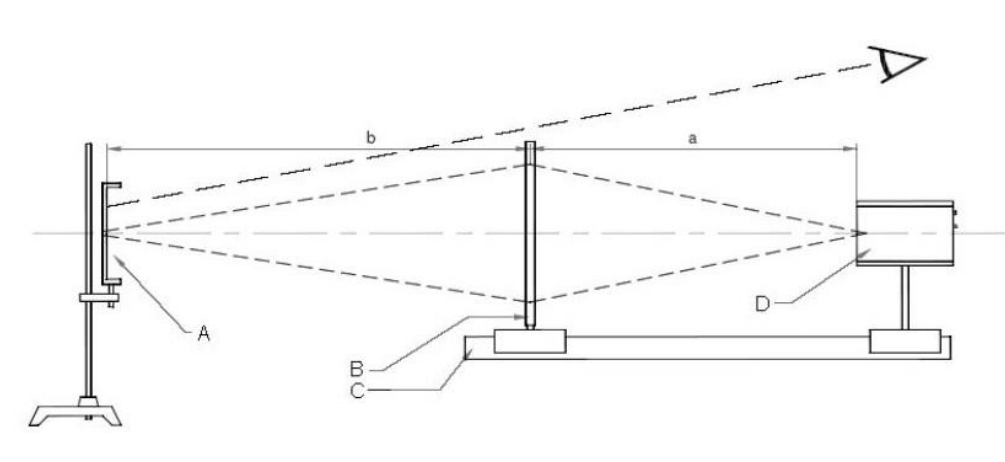
\includegraphics[width=10cm]{1}
				\vspace{2mm}
				\caption{Оптическая схема прибора для измерения скорости света}
				\label{fig:setup}
			\end{minipage}
		\end{center}
	\end{figure}
	
	\section{Порядок выполнения работы.}
	\begin{enumerate}
		\item Собрана оптическая схема на скамье модели U: установлены излучатель и приёмник прибора U8476460 на рейтерах U17160, выставлены их по оси скамьи.
		\item Схема подключена к прибору цифровой осциллограф PeakTech 1245;
		\item Измерено рулеткой положение приёмника относительно излучателя, задавая последовательно несколько значений $2S$;
		\item Для каждого положения $2S$ измерено по осциллографу время задержки $t$ измерительного импульса относительно референсного.
		\item Результаты занесены в табл.~\ref{tab:data}, $2S$ переведены в метры, а $t$ в секунды.
		\item По формуле \eqref{eq:1} расчитана скорость света для каждого опыта и среднее значение по формуле \eqref{eq:mean}.
		\item Построен график $2S(t)$, нанесены экспериментальные точки и проведена линейная аппроксимация; по наклону прямой определена скорость света.
		\item $c_{\text{ср}}$ сравнена с наклоном прямой и с табличным значением $c_0$, оценена относительную погрешность по формуле \eqref{eq:err}.
	\end{enumerate}
	
	\section{Ход выполнения работы.}
	
	\subsection{Таблицы с результатами прямых измерений и вычислений.}
	\begin{table}[H]
		\caption{Результаты измерений и вычислений}
		\label{tab:data}
		\centering
		\begin{tabular}{|c|c|c|c|c|}
			\hline
			№ измерения & \(2S\), см & \(2S\), м & \(t\), нс & \(t\), с \\
			\hline
			1 & 732 & 7.32 & 21.6 & \(2.16 \cdot 10^{-8}\) \\
			2 & 900 & 9.00 & 27.0 & \(2.70 \cdot 10^{-8}\) \\
			3 & 1059 & 10.59 & 31.8 & \(3.18 \cdot 10^{-8}\) \\
			4 & 1283 & 12.83 & 38.0 & \(3.80 \cdot 10^{-8}\) \\
			\hline
		\end{tabular}
	\end{table}
	
	По формуле \eqref{eq:1} рассчитывается скорость света для каждого опыта:
	\[
	c_1 = \frac{7.32}{2.16 \cdot 10^{-8}} \approx 3.3889 \cdot 10^8 \text{ м/с}
	\]
	\[
	c_2 = \frac{9.00}{2.70 \cdot 10^{-8}} \approx 3.3333 \cdot 10^8 \text{ м/с}
	\]
	\[
	c_3 = \frac{10.59}{3.18 \cdot 10^{-8}} \approx 3.3302 \cdot 10^8 \text{ м/с}
	\]
	\[
	c_4 = \frac{12.83}{3.80 \cdot 10^{-8}} \approx 3.3763 \cdot 10^8 \text{ м/с}
	\]
	
	Среднее значение скорости света по формуле \eqref{eq:mean}:
	\[
	c_{\text{ср}} = \frac{3.3889 + 3.3333 + 3.3302 + 3.3763}{4} \cdot 10^8 \approx 3.3572 \cdot 10^8 \text{ м/с}
	\]
	
	\subsection{Графики экспериментальных и расчётных зависимостей.}
	
	\begin{figure}[H]
		\centering
		\begin{tikzpicture}
			\begin{axis}[
				width=0.94\textwidth,
				height=8cm,
				axis lines=left,
				xlabel={$t$, нс},
				ylabel={$2S$, см},
				xmin=20.6, xmax=39.0,
				ymin=632, ymax=1320,
				xtick={20.6,22.6,24.6,26.6,28.6,30.6,32.6,34.6,36.6,38.6},
				ytick={632,832,1032,1232},
				tick label style={font=\small},
				label style={font=\normalsize},
				tick style={gray},
				axis line style={gray!65},
				clip=false,
				enlargelimits=false,
				]
				\addplot[
				only marks,
				mark=*,
				mark size=2.4pt,
				blue!75!black
				] coordinates {
					(21.6,732) (27.0,900) (31.8,1059) (38.0,1283)
				};
				\addplot[blue!65!black, thick, domain=20.6:39.0, samples=2]
				{33.600164*x - 1.06486};
				\node[anchor=north, align=center, font=\small] at (axis description cs:0.70,0.98)
				{$2S = 0{,}336\,t - 0{,}106$\\$R^2 = 0{,}9987$};
			\end{axis}
		\end{tikzpicture}
		\caption{Зависимость двойного пройденного расстояния $2S$ от времени задержки $t$ (наклон в см/нс численно равен $c$ в м/с)}
		\label{fig:distance-time}
	\end{figure}
	
	\section{Оценка ошибок измерений и вычислений.}
	
	Полученное среднее значение скорости света в воздухе:
	\[
	c_{\text{ср}} \approx 3.36 \cdot 10^8 \text{ м/с}.
	\]
	
	Относительная погрешность относительно табличного значения $c_0 = 2.9979 \cdot 10^8$ м/с по формуле \eqref{eq:err}:
	\[
	\delta = \frac{|3.3572 \cdot 10^8 - 2.9979 \cdot 10^8|}{2.9979 \cdot 10^8} \cdot 100\% \approx 11.98\%.
	\]
	
	\section{Выводы.}
	\subsection*{Анализ экспериментальных данных.}
	Импульсным методом получено $c_{\text{ср}} \approx 3{,}36 \cdot 10^8$ м/с. Зависимость $2S(t)$ линейна ($R^2 = 0{,}9987$), наклон $33{,}60$ см/нс даёт то же значение $c$, что и $c_{\text{ср}}$, что подтверждает модель $c = 2S/t$. Отклонение от $c_0$ --- около $12\%$.
	
	\subsection*{Сопоставление с теорией.}
	В воздухе $c \approx c_0/n$, $n \approx 1{,}0003$, т.е. отличие от $c_0$ не более $0{,}03\%$. Расхождение $\approx 12\%$ систематическое: наклон прямой и $c_{\text{ср}}$ совпадают.
	
	\subsection*{Критические замечания.}
	Причины расхождения: задержки электроники, погрешности рулетки ($\Delta(2S) \approx 0{,}5$ см) и осциллографа ($\Delta t \approx 0{,}2$ нс), неточность юстировки, отличие $n$ воздуха от вакуума. $R^2$ характеризует лишь линейность и систематику не устраняет; для повышения точности нужны калибровка задержки и увеличение базы $2S$. Цель достигнута.
	
	\newpage
	\section*{Список литературы}
	\addcontentsline{toc}{section}{Список литературы}
	
	\begin{enumerate}
		\item Алексеев В. П., Неменко Е. О., Рыбникова Е. В. Лабораторная работа № 12. Определение скорости света.~-- Ярославль: ЯрГУ, 2019.~-- 7~с.
		\item Сивухин, Д.~В. Курс общей физики~: в 5~т. Т.~5. Атомная и ядерная физика~: учебное пособие / Д.~В.~Сивухин.~-- 3-е изд., стер.~-- Москва~: ФИЗМАТЛИТ, 2002.~-- 784~с.~-- ISBN 5-9221-0230-4.
	\end{enumerate}
	
\end{document}